\documentclass[../main.tex]{subfiles}

\graphicspath{{../images/}}

\begin{document}
\pagestyle{fancy}
\lhead{Junseo Shin \& Jeremy Smith}
\rhead{Lab Notebook: Fourier Methods}
\chead{8/29/24}
% Day 1

\section*{Intro}
\addcontentsline{toc}{section}{Intro}


\paragraph*{The Three Experiment Timeline}
\begin{itemize}
    \item 7 Class sessions
    \item Signal recovery under noise: Ch 6 \& 15
    \item AM Radio Reception: Ch 3 \& 11
    \item The Fluxgate Magnometer: Ch 3 \& 13
\end{itemize}

\subsection{Familiarizing with Equipment (Chapter 0-2)}

Equipment list:
\begin{itemize}
    \item SR770 FFT Network Analyzer (main instrument)
    \item Keysight 33500B Waveform Generator (AC signal source) we will call 
    \item Tektronix TDS 1012 (oscilloscope/scope)
    \item Teach Spin Fourier Methods Electronic Modules (multi-tool)
    \item BNC (Bayonet-Neil-Concelman) cable: In short, a coaxial cable with default 50 ohm characteristic impedance for RF applications.
    All inputs and outputs will be connected via BNC cables.
\end{itemize}

% fig tmodule.png
\begin{figure*}[ht]
    \centering
    \includegraphics[width=\textwidth]{tmodule.png}
    \caption{Teach Spin Fourier Methods Electronic Modules}
\end{figure*}

\paragraph*{Fourier Series} (MAIN CONCEPT)

Any periodic function $f(t)$ with period $T$ can be expressed as a sum of sines and cosines:
\begin{align*}
    f(t) &= \frac{a_n}{2} + \sum_{n=1}^{\infty} a_n \cos(n\omega t) + b_n \sin(n\omega t)\\
    a_0 &= \frac{2}{T} \int_{0}^{T} f(t) dt\\
    a_n &= \frac{2}{T} \int_{0}^{T} f(t) \cos(n\omega t) dt\\
    b_n &= \frac{2}{T} \int_{0}^{T} f(t) \sin(n\omega t) dt
\end{align*}
where $\omega = 2\pi/T$ is the fundamental frequency and $n$ is the harmonic number. Or for voltage

\begin{align}
    V(t) &= V_{dc} + \sum_{n=1}^\infty \qt[C_n \cos(2\pi n t/T) + S_n \sin(2\pi n t/T)]
\end{align}
\paragraph*{Observations:}

\paragraph{For our first set of experiments we were simply trying to gain an understanding of the equipment and Fourier Analysis in general. We practiced by displaying several signals in the time and frequency domain using the oscilloscope and SSR770 repsectively.}
From the 33500B, output a 10 kHz, 1 V source to the SIGNAL IN of the SR770 with 
\begin{itemize}
    \item Simple sine wave: Selecting the Sine waveform on the 33500B, we can see the outputs in the time \& frequency domains
    as shown in Fig. \ref{fig:0.1} and \ref{fig:0.2}
    \begin{figure*}[ht]
        \centering
        \begin{minipage}{0.5\textwidth}
            \centering
            \includegraphics[width=\textwidth, page=8]{simple_waveform}
            \caption{TDS 1012 oscilloscope view}
            \label{fig:0.1}
        \end{minipage}\hfill
        \begin{minipage}{0.5\textwidth}
            \centering
            \includegraphics[scale=0.11, page=9]{simple_waveform}
            \caption{SR770 FFT Network Analyzer view}
            \label{fig:0.2}
        \end{minipage}
    \end{figure*}
    \newpage
    \item Square wave: Changing the waveform to SQUARE on the 33500B, we can intuit from the fourier series the coefficients are given by
    \begin{align*}
        a_0 &= 0 \\
        a_n &= 0 \\
        b_n &= \frac{4}{n\pi} \sin(n\pi/2)
    \end{align*}
    Thus the square wave is a sum of odd harmonics of the fundamental frequency with amplitudes
    \begin{align*}
        \qt[\frac{4}{\pi}, \frac{4}{3\pi}, \frac{4}{5\pi}, \frac{4}{7\pi}, \dots]
    \end{align*}
    for odd $n$ as shown in Fig. \ref{fig:0.4}.
    \begin{figure*}[ht]
        \centering
        \begin{minipage}{0.5\textwidth}
            \centering
            \includegraphics[width=\textwidth, page=6]{simple_waveform}
            \caption{TDS 1012 oscilloscope view}
            \label{fig:0.3}
        \end{minipage}\hfill
        \begin{minipage}{0.5\textwidth}
            \centering
            \includegraphics[scale=0.11, page=7]{simple_waveform}
            \caption{SR770 FFT Network Analyzer view}
            \label{fig:0.4}
        \end{minipage}
    \end{figure*}
    In Fig. \ref{fig:0.3} we can see the shape of the waveform in the time domain,
    and the odd harmonics are clearly shown in the SR770 frequency domain (Fig. \ref{fig:0.4}). 

    \newpage
    \item Saw Wave: (SAW waveform on 33500B) The saw wave is a sum of all harmonics of the fundamental frequency as shown in Fig. \ref{fig:0.6}.
    \begin{figure*}[ht]
        \centering
        \begin{minipage}{0.45\textwidth}
            \centering
            \includegraphics[width=\textwidth, page=4]{simple_waveform}
            \caption{TDS 1012 oscilloscope view}
            \label{fig:0.5}
        \end{minipage}\hfill
        \begin{minipage}{0.45\textwidth}
            \centering
            \includegraphics[scale=0.11, page=5]{simple_waveform}
            \caption{SR770 FFT Network Analyzer view}
            \label{fig:0.6}
        \end{minipage}
    \end{figure*}

    \item Triangle Wave: (TRIANGLE waveform on 33500B) The triangle wave is a sum of all odd harmonics of the fundamental frequency as shown in Fig. \ref{fig:0.8}.
    \begin{figure*}[ht]
        \centering
        \begin{minipage}{0.45\textwidth}
            \centering
            \includegraphics[width=\textwidth, page=1]{simple_waveform}
            \caption{TDS 1012 oscilloscope view}
            \label{fig:0.7}
        \end{minipage} \hfill
        \begin{minipage}{0.45\textwidth}
            \centering
            \includegraphics[width=0.8\textwidth, page=2]{simple_waveform}
            \caption{SR770 FFT Network Analyzer view}
            \label{fig:0.8}
        \end{minipage}\hfill
    \end{figure*}
    But the amplitude of the harmonics decreases by a factor of $1/n^2$. This power law makes the amplitude hard to read in the linear scale,
    but in the log scale, the amplitudes are clearly visible as shown in Fig. \ref{fig:0.9}.
    \begin{figure*}[ht]
        \centering
        \includegraphics[width=0.5\textwidth, page=3]{simple_waveform}
        \caption{SR770 LOG MAGNITUDE}
        \label{fig:0.9}
    \end{figure*}

\end{itemize}

\newpage

\paragraph*{Superposition of sine waves}

\begin{itemize}
    \item 770: 40 kHz, 1 V sine wave $\to$ SUMMER input A
    \item 33500B: 50 kHz, 2 V sine wave $\to$ SUMMER input B
    \item SUMMER output $\to$ 770 SIGNAL IN \& TDS 1012
\end{itemize}

\begin{figure*} [ht]
    \centering
    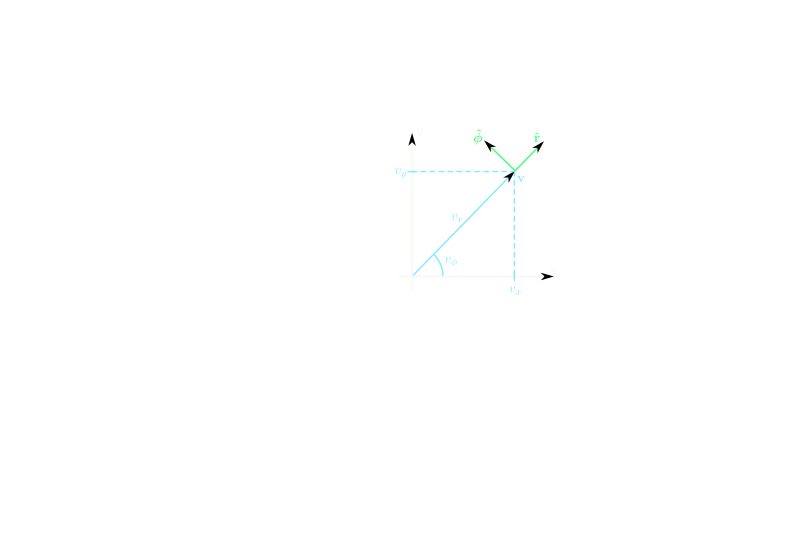
\includegraphics[width=0.5\textwidth]{fig1.png}
    \caption{Diagram of setup}
\end{figure*}

From the 770, we can easily see the two sine waves in the frequency domain as shown in Fig. [insert fig 0.11],
but the time domain (scope) does not clearly describe the summation of the two waves.

\paragraph*{Similar amplitude}
\begin{itemize}
    \item 770: 50 kHz, 1 V sine wave $\to$ SUMMER input A
    \item 33500B: 51 kHz, 1 V sine wave $\to$ SUMMER input B
\end{itemize}

In the full (100 kHz) span view, we can't see the two peaks.
To increase the frequency resolution, we can reduce the span in the 770 FREQ menu, 
but this will increase the acquisition time. 

e.g. a full span of 100 kHz has an acquisition time of 4 ms;
the `voltage sampling' rate is 256 kSa/s, or 256 samples per ms i.e. 1024 samples in 4 ms.

For our experiment, we set the span to 1.56 kHz to clearly see the two peaks, but this costs us
an acquisition time of 256 ms or $256 * \qty{256}{samples/ms} = 65536$ samples. This trade-off can be described by
the `frequency duration uncertainty principle':

\[\textrm{(frequency resolution achievable)} \cdot \textrm{(acquisition time required)} \geq  \textrm{a number}\]

The 770 magic number is
\begin{align*}
    \qty{100}{kHz} \cdot \qty{4}{ms} &\geq \qty{400}{kHz.ms}
\end{align*}
which we can use to find the minimum acquisition time for a given frequency resolution e.g. the 1.5625 kHz span required
\begin{align*}
    \textrm{(acquisition time req)} &\geq 400 / \textrm{(freq resolution)} \\
    &= 400 / 1.5625 = \qty{256}{ms}
\end{align*}

\paragraph*{Windowing \& Different amplitude}

Recommended windowing:
\begin{itemize}
    \item Uniform: close spaced peaks with similar amplitudes
    \item Flattop: accurate peak height measurement
    \item Hanning: good for spectral resolution
    \item BMH: good for weak peak near strong peak, but not the best resolution for top peak \& amplitude accuracy
\end{itemize}

\subsubsection*{Summary} 

We have learned the basic concepts of Fourier series and the Fourier transform, and analyzed basic waveforms from the 33500
in both the time and freqency domains using the scope and 770 respectively.
Furthermore, there are trade offs between frequency resolution and acquisition time,
and the choice of windowing function which can affect the accuracy of the measurement.
\newpage
\chead{9/3/24-9/5/24}
\section{Signal Recovery Under Noise}

\subsection*{Chapter 6: Noise Waveforms}
\addcontentsline{toc}{subsection}{Chapter 6: Noise Waveforms}

After reading chapters 6 \& 15 we will be proceeding with the Signal Recovery from under noise experiment. We will be attempting to locate an unknown signal amongst some random noise.

\paragraph*{Initial Setup}

T-Spin's ``buried treasure'' (BT) module through a F splitter to both the ‘scope and the SR770 as shown in Fig. \ref{fig:1.1} and \ref{fig:1.2}.

% fig1_1a.png and fig1_1b.png
\begin{figure*}[ht]
    \centering
    \begin{minipage}{0.5\textwidth}
        \centering
        \includegraphics[width=0.8\textwidth]{fig1_1a.jpg}
        \caption{BT Noise on scope (Time Domain)}
        \label{fig:1.1}
    \end{minipage}\hfill
    \begin{minipage}{0.5\textwidth}
        \centering
        \includegraphics[width=\textwidth]{fig1_1b.jpg}
        \caption{BT Noise on SR770 (Frequency domain)}
        \label{fig:1.2}
    \end{minipage}
\end{figure*}

Changing the rotary switch on the BT module to ``filtered noise'' (\ref{fig:0.1}) will
filter out all frequencies about the full span of the 770, i.e., all frequencies above 100 kHz will be filtered out which is shown in Fig. \ref{fig:1.3} and \ref{fig:1.4}.

% fig1_3a.png and fig1_3b.png
\begin{figure*}[ht]
    \centering
    \begin{minipage}{0.5\textwidth}
        \centering
        \includegraphics[width=\textwidth]{fig1_3.jpg}
        \caption{Filtered Noise on scope}
        \label{fig:1.3}
    \end{minipage}\hfill
    \begin{minipage}{0.5\textwidth}
        \centering
        \includegraphics[width=\textwidth]{fig1_4.jpg}
        \caption{Filtered Noise on SR770}
        \label{fig:1.4}
    \end{minipage}
\end{figure*}

\newpage
\paragraph*{}
By averaging out the noise using 64 averages we achieved a flat waveform, demonstrating that the power spectrum for white noise, because it is statistically random, is flat across frequencies.
The 64 in this case, refers to the idea that during acquisition we are taking an average for ever 4 ms

% fig1_5.png
\begin{figure*}[ht]
    \centering
    \includegraphics[width=0.8\textwidth]{fig1_5.jpg}
    \caption{Filtered Noise on SR770 with 64 averages}
    \label{fig:1.5}
\end{figure*}

We then switched the noise to “pink” noise and averaged out the waveform to its power spectrum.

% fig1_6.png
\begin{figure*}[ht]
    \centering
    \includegraphics[width=0.8\textwidth]{fig1_6.jpg}
    \caption{Pink Noise on SR770 with 64 averages}
    \label{fig:1.6}
\end{figure*}

In attempting to record the $V_\text{rms}$ for a monochromatic 1 V, 50 kHz sinusoidal wave,
we erroneously plug our BNC cable into the sync output of the waveform generator and saw a square wave.
Which makes sense due to information rates being in binary format.

\newpage
We eventually recorded the power spectrum of a monochromatic sinusodial wave of 1 V and 50 kHz (\ref{fig:1.7}), and the $V_\text{rms} = 0.707$ V as measured
by the scope. 

% fig1_7.png
\begin{figure*}[ht]
    \centering
    \includegraphics[width=0.8\textwidth]{fig1_7.jpg}
    \caption{1 V, 50 kHz sinusoidal wave on SR770}
    \label{fig:1.7}
\end{figure*}

\paragraph*{Measuring RMS Voltage of Noise}
For white noise, to find the mean square measure of voltage we must take the Power spectral density $PSD = VSD^2$ and integrate over the frequency space:

\begin{align*}
    \int_0^\infty S(f) df &= \langle V^2(t) \rangle
\end{align*}
So in the case of white noise (Fig. \ref{fig:1.7})
\begin{align*}
    \int_0^{\qty{100}{kHz}} S(f) df &= PSD * (\textrm{Frequency Range}) = \qt(\frac{\qty{244}{\micro V}}{\sqrt{\text{Hz}}})^2 * \qty{100}{kHz} = \qty{5.96e-3
    }{V}
\end{align*}

Furthermore, we know the relation of mean-square voltage and the total power:
\begin{align*}
    V_\text{rms} = \sqrt{\langle V^2(t) \rangle} = 0.0772 V
\end{align*}

\newpage
\subsection*{Noise Plus Sine Wave}

\paragraph*{Experiment Part 1: Setup} The Signal Pipeline TM:

BT Filtered Noise or Buried Signal $\to$ WIDE BAND AMP 25x $\to$ Low Pass 20 kHz, $Q=0.71 \to $ Summer adding Sine 10kHz, 0.3 V (Output off initially).

\paragraph*{770 Config}

\begin{itemize}
    \item SPAN: 195 Hz
    \item AVERAGES: 64 (2.048 s)
    \item MEASure: PSD (actually VSD but the 770 calls it PSD)
    \item WINDOW: Flattop (for peak amplitude)
    \item Display: Log Magnitude
    \item CENTER Freq. 10 kHz
\end{itemize}

\begin{figure}[ht]
    \includegraphics[width=\textwidth]{exp1_1.png}
    \caption{Control setup for Signal Under Noise}
    \label{fig:exp1}
\end{figure}

\paragraph*{Pre Trial Observations} Scope vs. 770

The scope obviously shows a noise signal where we can't see the sine wave, but the 770 clearly shows the sine wave as shown in Fig. \ref{fig:1.8}.

% fig1_8.png
\begin{figure*}[ht]
    \centering
    \includegraphics[width=0.8\textwidth]{fig1_8.jpg}
    \caption{Sine wave on SR770 with noise}
    \label{fig:1.8}
\end{figure*}

\newpage
\paragraph*{Procedure}

% fig1_9.png and fig1_10.png
\begin{figure*}[ht]
    \centering
    \begin{minipage}{0.45\textwidth}
        \centering
        \includegraphics[width=\textwidth]{fig1_9.jpg}
        \caption{Filtered Noise with Sine wave on SR770}
        \label{fig:1.9}
    \end{minipage}\hfill
    \begin{minipage}{0.45\textwidth}
        \centering
        \includegraphics[width=\textwidth]{fig1_10.jpg}
        \caption{Filtered Noise without Sine wave on SR770}
        \label{fig:1.10}
    \end{minipage}
\end{figure*}

\begin{itemize}
    \item With the sine wave off (Fig \ref{fig:1.10}), take a sample of the VSD at $5, 10, 15, 20$ kHz in order to calculate the average VSD of the noise floor.
    We have removed 0 Hz from the calculation as VSD goes to infinity as it approaches 0 Hz.
    \item Meausre $\langle V_n^2 \rangle$ using the equation for relating the spectral density to the mean-square voltage:
    \begin{align*}
        \langle V_n^2 \rangle = \int_0^\infty S(f) df = PSD * (\textrm{Frequency Range}) = VSD^2 * \qty{20}{kHz}
    \end{align*}
    \item Measure the mean-square measure of the signal sine wave $\langle V_s^2 \rangle$ by connecting the sine signal directly to the 770 and measuring the $V_\text{rms}$ using the Voltz rms UNITS menu \& 64 Averages.
    \item Calculate the predict the measure of the signal (sine wave) $V_s$ plus noise $V_n$ using
    \begin{align*}
        \langle \qt[
            V_s + V_n
        ]^2 \rangle &= \langle V_s^2 \rangle + \langle V_n^2 \rangle = \langle V_T^2 \rangle
    \end{align*}
    where the cross terms are zero since the signal and noise are independent of each other.
    \item Measure $\langle V_T^2 \rangle$ using the TDS1012 scope and calculate the average for 20 samples for the Signal plus noise input:
    \begin{itemize}
        \item Finding rms voltage on scope: Go to SETTINGS; AQCUIRESE; SAMPLE; AVERAGE (16). Then take 20 samples and average them (refer to Fig. \ref{fig:1.11}).
    \end{itemize}
    \item Check if the measured value is within the predicted value. Then calculate how much of the signal plus waveform is due to the signal from a power basis i.e. 
    \begin{align*}
        \% \text{ Signal} = \frac{\langle V_s^2 \rangle}{\langle V_T^2 \rangle} * 100\%
    \end{align*}
    \item Repeat two more trial but with WIDEBAND AMP ($1 \times 1 \times 2.5 = 2.5$) and with Sine wave at 1 V (25x WIDEBAND AMP).
\end{itemize}

\begin{figure*}[ht]
    \centering
    \includegraphics[width=0.55\textwidth]{fig1_11.jpg}
    \caption{Sample measurement of $V_T = \qty{642}{mV}$ on TDS1012}
    \label{fig:1.11}
\end{figure*}

\newpage
\subsubsection*{Data}

\begin{table}[!ht]
    \centering
    \begin{tabular}{|c|l|l|l|}
    \hline
        Freq (Hz) & Trial 1 (mV/$\sqrt{\text{Hz}}$) & Trial 2 (mV/$\sqrt{\text{Hz}}$) & Trial 3 (mV/$\sqrt{\text{Hz}}$) \\ \hline
        5 & 4.635 & 0.4759 & 4.268 \\ \hline
        10 & 4.52 & 0.4298 & 4.306 \\ \hline
        15 & 4.174 & 0.4145 & 3.853 \\ \hline
        20 & 3.193 & 0.307 & 3.201 \\ \hline
        Avg & 4.1 & 0.41 & 3.9 \\ \hline
        STD ($\pm$ mV) & 0.7 & 0.07 & 0.5 \\ \hline
        Signal $V_s$ (mV) & 207.1 & 208.8 & 703.9 \\ \hline
    \end{tabular}
    \caption{770 measurements for Average $V_\text{rms}$ for Noise and Signal}
    \label{tab:1}
\end{table}

\begin{table}[!ht]
    \centering
    \begin{tabular}{|c|l|l|l|}
    \hline
        Sample & Trial 1 (mV) & Trial 2 (mV) & Trial (V) \\ \hline
        1 & 834 & 218 & 1.69 \\ \hline
        2 & 845 & 187 & 0.759 \\ \hline
        3 & 468 & 191 & 1.34 \\ \hline
        4 & 787 & 252 & 0.851 \\ \hline
        5 & 389 & 244 & 0.964 \\ \hline
        6 & 745 & 213 & 0.95 \\ \hline
        7 & 532 & 213 & 0.633 \\ \hline
        8 & 635 & 257 & 0.879 \\ \hline
        9 & 725 & 220 & 1.22 \\ \hline
        10 & 523 & 249 & 1.4 \\ \hline
        11 & 960 & 197 & 0.588 \\ \hline
        12 & 401 & 223 & 1.17 \\ \hline
        13 & 676 & 249 & 0.857 \\ \hline
        14 & 380 & 189 & 1.1 \\ \hline
        15 & 749 & 204 & 0.812 \\ \hline
        16 & 512 & 208 & 0.817 \\ \hline
        17 & 621 & 163 & 0.796 \\ \hline
        18 & 625 & 169 & 0.942 \\ \hline
        19 & 528 & 232 & 0.683 \\ \hline
        20 & 672 & 235 & 1.32 \\ \hline
        AVG (V) & 0.6 & 0.22 & 1.0 \\ \hline
        STD ($\pm$ V) & 0.2 & 0.03 & 0.3 \\ \hline
    \end{tabular}
    \caption{Scope measurements for $V_T$}
    \label{tab:2}
\end{table}

Example calculation for the rms measure of the signal plus noise in Trial 1:
\begin{align*}
    \langle V_n^2 \rangle &= PSD * \Delta f  = \qt(\qty{4.1}{mV/\sqrt{Hz}})^2 * \qty{20}{kHz} = \qty{0.34}{V} \\
    \langle V_s^2 \rangle &= \qty{207.1}{mV}^2 = \qty{0.04}{V} \\
    \langle V_T^2 \rangle &= \qty{0.34}{V} + \qty{0.04}{V} = \qty{0.38}{mV} \\
    V_T &= \sqrt{\qty{0.38}{V}} = \qty{0.62}{V}
\end{align*}
and error
\begin{align*}
    \delta V_n = 2 * \qty{0.7e-3}{V/\sqrt{Hz}} * \qty{20000}{Hz} = 30 \implies \delta V_T = \frac{1}{2} * 30 = 15 V
\end{align*}
The error bars on the 770 measurements are not very useful here since we are propogating the average spectral density based on only 4 frequencies (5, 10, 15, 20 Hz) onto 20,000 Hz.
So we will rather use the error bars from the scope measurement and ignore the 770 error bars.

\begin{table}[!ht]
    \centering
    \begin{tabular}{|c|l|l|l|}
    \hline
        & Trial 1 & Trial 2 & Trial 3 \\ \hline
        $V_n^2$ & 0.341 & 0.0033 & 0.305 \\ \hline
        $V_s^2$ & 0.043 & 0.0436 & 0.495 \\ \hline
        $V_T^2$ & 0.384 & 0.0469 & 0.801 \\ \hline
        $V _T$ & 0.62 & 0.22 & 0.89 \\ \hline
        \% Signal & 11\% & 93\% & 62\% \\ \hline
    \end{tabular}
    \caption{Voltage measurements and Percent of Power due to Signal}
    \label{tab:3}
\end{table}

\paragraph*{Quick Analysis of Data}
As we compare the data from Table \ref{tab:2} and Table \ref{tab:3}, all the measured values are within the predicted values, and the \% signal is within the expected range stated 
in the Teach Spin manual for Trial 1 (11\%).

\paragraph*{Summary}
So we were able to successfully measure the mean-square voltage of the signal plus noise using the 770 and the scope.
The weird unit of interest $V/\sqrt{\text{Hz}}$, the voltage spectral density, becomes a useful tool to measure noise and delineate 
the signal from the noise. (9/5/24) Trial 2 clearly shows a smaller noise floor presents a clearer signal defined by the percent of signal power,
and vice versa for Trial 3 and a larger sine wave amplitude.

\newpage
\chead{9/5/24}
\subsection*{Chapter 15: Signal Recovery Under Noise}
\addcontentsline{toc}{subsection}{Chapter 15: Signal Recovery Under Noise}

\paragraph*{Experiment Part 2:} Signal Pipeline TM:

BT Noise (A, B, C, or D) $\to$ SR770

\paragraph*{770 Config}
\begin{itemize}
    \item AVERAGE: 16 Exponential mode (for now)
    \item MEASure: PSD (Actually VSD but the 770 calls it PSD)  
    \item WINDOW: Uniform for close peaks with similar amplitudes, Flattop for measurment
\end{itemize}

% exp1_2.png
\begin{figure*}[ht]
    \centering
    \includegraphics[width=0.8\textwidth]{exp1_2.png}
    \caption{Buried Treasure Setup}
    \label{fig:exp1_2}
\end{figure*}

\paragraph*{Notes from Teach Spin} Inexact Calculation of 
\begin{itemize}
    \item 770 sorts frequencies into 400 bins of width $\delta f$, so any bin with just noise has expected value
    \begin{align*}
        \langle V_n^2 \rangle = \int S(f) df \to S \delta f
    \end{align*}
    compared to an expected value of the signal (plus some noise) has expected value
    \begin{align*}
        \langle \qt[V_(t) + A \cos(\omega t -\phi)]^2 \rangle = S \delta f + \frac{A^2}{2} = \langle V_P^2 \rangle
    \end{align*}
    thus we need signal power in a single bin to be much larger than the STD of noise floor values in the bin. 
    \item To find and $N$ standard deviation detection of the signal with $n$ acquisitions (or Averages) the noise of the bin must be smaller than
    \begin{align*}
        \frac{A^2}{2} > N \frac{S \delta f}{\sqrt{n}}
    \end{align*}
    e.g. $N = 5$-sigma detecti on of the signal with $n = 16$ Average. 
\end{itemize}

\paragraph*{Procedure}
\begin{itemize}
    \item Turn the Rotary switch to buried signal A and output the signal \textit{directly} to the 770.
    \item Decrease the Frequncy span to the next smaller value and use exponential average to look for a peak that stands up atleast 20 dB above the noise floor.
    \item Repeatedly decrease the span and pan through the full range of the 770 until you find the peak. 
    \item Once the peak is found, measure the peak voltage using the MEASure: Spectrum; Units: Voltz Pk.
    \item If the peak does not stand out as far, subtract the mean square power per bin (PSD per bin) between the peak $V_P$ an an only-noise bin $V_n$ i.e.
    \begin{align*}
        \frac{A^2}{2} = \langle V_P^2 \rangle - \langle V_n^2 \rangle
    \end{align*}
\end{itemize}

\begin{table}[!ht]
    \centering
    \begin{tabular}{|c|c|c|}
    \hline
        BT Signal & A (freq) & V\_P (mV) \\ \hline
        A & 2.875 kHz & 15.62 \\ \hline
        B & 70.26 kHz & 6.466 \\ \hline
        C & 33.57 kHz & 1.46 \\ \hline
    \end{tabular}
    \caption{Measured Frequency and Peak Voltage for BT Signal}
    \label{tab:4}
\end{table}

\begin{figure*}[!ht]
    \centering
    \includegraphics[width=0.8\textwidth]{fig1_12.jpg}
    \caption{770 View for BT Signal C}
    \label{fig:1.12}
\end{figure*}

\paragraph*{Summary}
From Fig. \ref{fig:1.12} We had to pan through the full range of the 770 at $100 / 2^6 = 1.5625$ kHz to find the peak at 33.57 kHz.
This means that we had todecrease the span 6 times to find the peak, and comb through each \~1.5 kHz range and wait for the 770 to acquire $n$ average each time.
Since the 770 cannot analyze the full span at small frequency ranges all at once, we had to manually pan through the full range for each iteration. 
Finally, we chose not to look for Signal D as it was only limited by the time it would have taken to pan through the full range of the 770 at even
smaller frequency ranges and larger averaging.
\end{document}